%%%%%%%%%%%%%%%%%%%%%%%%%%%%%%%%%%%%%%%%%
% Beamer Presentation
% LaTeX Template
% Version 1.0 (10/11/12)
%
% This template has been downloaded from:
% http://www.LaTeXTemplates.com
%
% License:
% CC BY-NC-SA 3.0 (http://creativecommons.org/licenses/by-nc-sa/3.0/)
%
%%%%%%%%%%%%%%%%%%%%%%%%%%%%%%%%%%%%%%%%%

%----------------------------------------------------------------------------------------
%	PACKAGES AND THEMES
%----------------------------------------------------------------------------------------

\documentclass{beamer}

\mode<presentation> {

% The Beamer class comes with a number of default slide themes
% which change the colors and layouts of slides. Below this is a list
% of all the themes, uncomment each in turn to see what they look like.

\usetheme{default}
%\usetheme{AnnArbor}
%\usetheme{Antibes}
%\usetheme{Bergen}
%\usetheme{Berkeley}
%\usetheme{Berlin}
%\usetheme{Boadilla}
%\usetheme{CambridgeUS}
%\usetheme{Copenhagen}
%\usetheme{Darmstadt}
%\usetheme{Dresden}
%\usetheme{Frankfurt}
%\usetheme{Goettingen}
%\usetheme{Hannover}
%\usetheme{Ilmenau}
%\usetheme{JuanLesPins}
%\usetheme{Luebeck}
%\usetheme{Madrid}
%\usetheme{Malmoe}
%\usetheme{Marburg}
%\usetheme{Montpellier}
%\usetheme{PaloAlto}
%\usetheme{Pittsburgh}
%\usetheme{Rochester}
%\usetheme{Singapore}
%\usetheme{Szeged}
%\usetheme{Warsaw}

% As well as themes, the Beamer class has a number of color themes
% for any slide theme. Uncomment each of these in turn to see how it
% changes the colors of your current slide theme.

%\usecolortheme{albatross}
\usecolortheme{beaver}
%\usecolortheme{beetle}
%\usecolortheme{crane}
%\usecolortheme{dolphin}
%\usecolortheme{dove}
%\usecolortheme{fly}
%\usecolortheme{lily}
%\usecolortheme{orchid}
%\usecolortheme{rose}
%\usecolortheme{seagull}
%\usecolortheme{seahorse}
%\usecolortheme{whale}
%\usecolortheme{wolverine}

%\setbeamertemplate{footline} % To remove the footer line in all slides uncomment this line
\setbeamertemplate{footline}[page number] % To replace the footer line in all slides with a simple slide count uncomment this line

%\setbeamertemplate{navigation symbols}{} % To remove the navigation symbols from the bottom of all slides uncomment this line
}

\usepackage{graphicx} % Allows including images
\usepackage{booktabs} % Allows the use of \toprule, \midrule and \bottomrule in tables
\usepackage{cancel}
\usepackage{amsmath,amssymb}
\beamertemplatenavigationsymbolsempty

\usepackage{tikz}
\usetikzlibrary{shapes,arrows,shapes.multipart}
\newcommand{\der}[2]{\frac{\partial #1}{\partial #2}}

\usepackage{lmodern}
\usepackage[T1]{fontenc}

%----------------------------------------------------------------------------------------
%	TITLE PAGE
%----------------------------------------------------------------------------------------


\title{\scshape Aaaaaaa}
\subtitle{Chapter 2: Overview of the Financial System}
\author{ \large XXXXX}

\institute[AAAAAAA] % Your institution as it will appear on the bottom of
% every slide, may be shorthand to save space
{
 \\ % Your institution for the title page
}
\date{july} % Date, can be changed to a custom date

\begin{document}

\begin{frame}
\titlepage % Print the title page as the first slide
\end{frame}




%----------------------------------------------------------------------------------------
%	PRESENTATION SLIDES
%----------------------------------------------------------------------------------------

%------------------------------------------------
%\section{Introduction} % Sections can be created in order to organize your presentation into discrete blocks, all sections and subsections are automatically printed in the table of contents as an overview of the talk
%------------------------------------------------

\begin{frame}
\frametitle{Function of Financial Markets}
\begin{itemize}
\item Channels funds from person or business without investment opportunities (i.e., "Lender-Savers") to one who needs funds to finance their spending (i.e., "Borrower-Spenders")
\vspace{\baselineskip}
\item Improves economic efficiency
\end{itemize}
\end{frame}


%------------------------------------------------

\begin{frame}
\frametitle{Financial Markets Funds Transferees}
\begin{itemize}
\item Lender-Savers
\begin{enumerate}
\item Households
\item Business firms
\item Government
\item Foreigners
\end{enumerate}

\vspace{\baselineskip}

\item Borrower-Spenders
\begin{enumerate}
\item Business firms
\item Government
\item Households
\item Foreigners
\end{enumerate}

\end{itemize}
\end{frame}


%------------------------------------------------

\frame
{
\frametitle{Flows of Funds Through the Financial System}
\centering 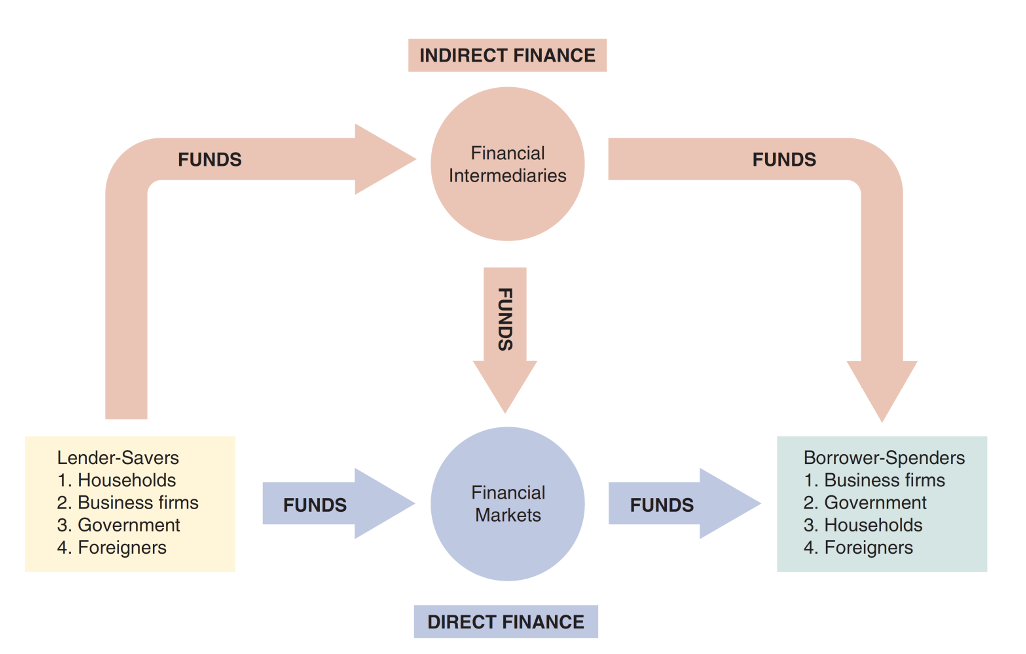
\includegraphics[height=8cm,width=12cm]{Picture1}
}
%------------------------------------------------
\begin{frame}
\frametitle{Function of Financial Markets}
\begin{itemize}
\item Direct Finance \\
\smallskip
Borrowers borrow directly from lenders in financial markets by selling securities (financial instruments) which are claims on the borrower's future income or assets. \\
Securities are \textbf{assets} for the person who buys them, but they are \textbf{liabilities} (IOUs or debts) for the person who sells (issues) them. 
\smallskip
\item bond: a debt security that promises to make payments periodically for a specified period of time
\item stock: a security that entitles the owner to a share of the company's profits and assets
\end{itemize}
\end{frame}


%------------------------------------------------
\begin{frame}
\frametitle{Function of Financial Markets}
\begin{itemize}
\item Indirect Finance \\
\smallskip
Borrowers borrow indirectly from lenders via financial intermediaries (established to source both loanable funds and loan opportunities) by issuing financial instruments which are claims on the borrower's future income or assets

\end{itemize}
\end{frame}



%------------------------------------------------
\begin{frame}
\frametitle{Importance of Financial Markets}
\begin{itemize}
\item For example, if you save \$1,000, but there are no financial markets, then you can earn no return on this - might as well put the money under your mattress.
\vspace{\baselineskip}
\item However, if a carpenter could use that money to buy a new saw (increasing her productivity), then she is willing to pay you some interest for the use of the funds.
\vspace{\baselineskip}
\item Financial markets are critical for producing an efficient allocation of capital, allowing funds to move from people who lack productive investment opportunities to people who have them.
\vspace{\baselineskip}
\item Financial markets also improve the well-being of consumers, allowing them to time their purchases better (e.g. buy a house when young, pay back over time).
\end{itemize}
\end{frame}


%------------------------------------------------
\begin{frame}
\frametitle{Structure of Financial Markets }

\begin{enumerate}
\item Debt Markets
\smallskip
\begin{itemize}
\item Debt instrument (e.g. bond, mortgage): is a contractual agreement by the borrower to pay the holder of the instrument fixed amounts at regular intervals (interest and principle payments) until a specified date (the maturity date) when a final payment is made.
\item Short-Term (maturity <  1 year)
\item Long-Term (maturity > 10 year)
\item Intermediate term (maturity in-between)
\end{itemize}
\vspace{\baselineskip}

\item Equity Markets
\smallskip
\begin{itemize}
\item Equities (e.g. common stocks): claims to share in the net income and the assets of a business. 
\item Pay dividends (periodic payments), in theory forever, long term securities
\item Represents an ownership claim in the firm
\item An equity holder is a \textit{residual claimant}, corporations must pay debt holders before equity holders
\end{itemize}
\end{enumerate}
\end{frame}

%------------------------------------------------
\begin{frame}
\frametitle{Structure of Financial Markets }

\begin{enumerate}
\item Primary Market
\smallskip
\begin{itemize}
\item New security issues sold to initial buyers
\item Typically involves an investment bank who underwrites the offering (guarantees a price for a corporation's securities and then sells them to the public) 
\end{itemize}

\end{enumerate}
\end{frame}



\begin{frame}
\frametitle{Structure of Financial Markets }

\begin{enumerate}

\item Secondary Market
\smallskip
\begin{itemize}
\item Securities previously issued are bought and resold
\item stock markets such as the NYSE and NASDAQ, bond markets, foreign exchange markets, future markets, options markets
\item Involves both brokers and dealers
\item Brokers are agents of investors who match buyers with sellers of securities
\item Dealers link buyers and sellers by buying and selling securities at stated prices
\item Corporation that issued the security acquires no new funds

\end{itemize}
\end{enumerate}
\end{frame}

%------------------------------------------------

\begin{frame}
\frametitle{Structure of Financial Markets }

Even though firms don't get any money, per se, from the secondary market, it serves two important functions:
\smallskip
\begin{itemize}
\item Provides liquidity, making it easy to buy and sell the securities of the companies
\item Establishes a price for the securities (useful for company valuation)
\end{itemize}

\end{frame}

%------------------------------------------------
\begin{frame}
\frametitle{Structure of Financial Markets }

We can further classify secondary markets as follows:
\vspace{\baselineskip}

\begin{enumerate}
\item Exchanges
\smallskip
\begin{itemize}
\item Trades conducted in central locations (e.g., New York Stock Exchange, Chicago Board of Trade)
\item the examples for Turkey? \textcolor{red}{(homework! not to be collected but may come up in quizzes and exams)}
\end{itemize}
\vspace{\baselineskip}

\item Over-the-Counter Markets
\smallskip
\begin{itemize}
\item Dealers at different locations buy and sell
\item Best example is the market for Treasury Securities
\end{itemize}
\end{enumerate}
\end{frame}

%------------------------------------------------
\begin{frame}
\frametitle{Classifications of Financial Markets}

\begin{enumerate}
\item Money Market: Short-Term (maturity < 1 year) debt instruments, more liquid, safer (smaller fluctuations in prices)
\smallskip

\item Capital Market: Long-Term (maturity > 1 year) debt plus equities (no maturity)

\end{enumerate}
\end{frame}

%------------------------------------------------

\begin{frame}
\frametitle{Internationalization of Financial Markets }

The internationalization of markets is an important trend. The U.S. no longer dominates the world stage.
\smallskip
\begin{itemize}
\item International Bond Market \& Eurobonds
\begin{itemize}
\item Foreign bonds: Denominated in a foreign currency, targeted at a foreign market
\item Eurobonds: Denominated in one currency, but sold in a different market, over 80 \% of new bonds are Eurobonds
\end{itemize}

\item Eurocurrency Market
\begin{itemize}
\item Foreign currency deposited outside of home country
\item Eurodollars are U.S. dollars deposited, say, London.
\item short term deposits earn interest, gives US an alternative source for dollars.
\end{itemize}

\item World Stock Markets
\begin{itemize}
\item U.S. stock markets are no longer always the largest - at one point, Japan's was larger
\end{itemize}

\end{itemize}

\end{frame}


%------------------------------------------------

\frame
{
\frametitle{ }
\centering 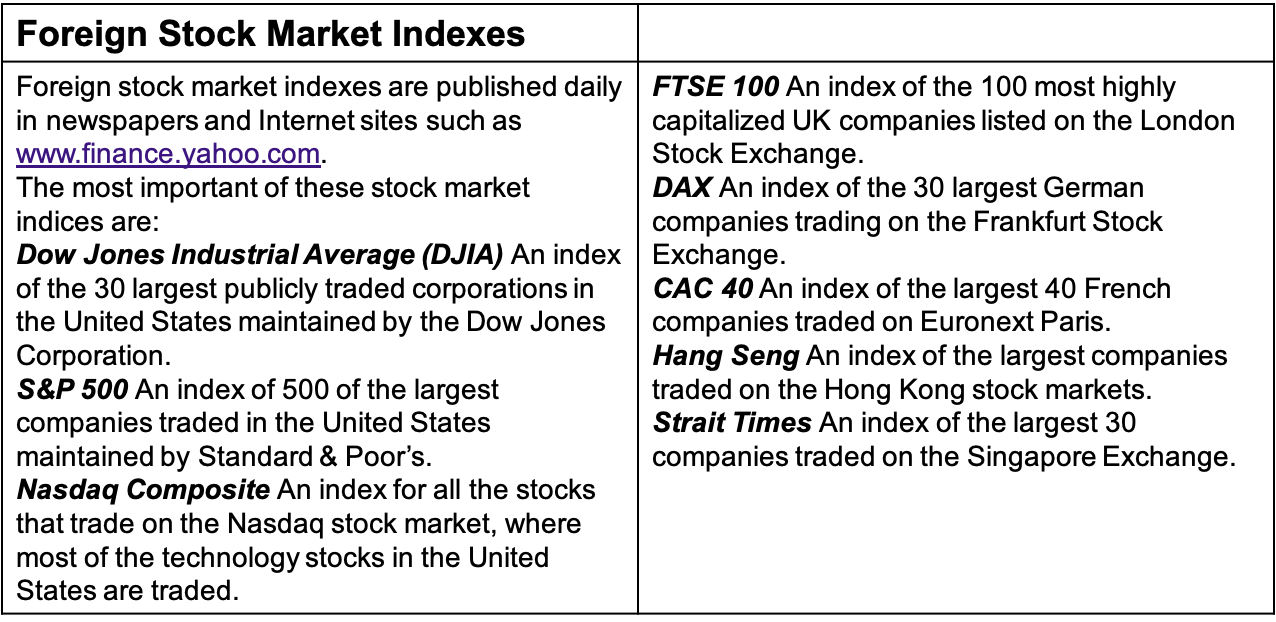
\includegraphics[height=7cm,width=11cm]{Picture2}
}


%------------------------------------------------
\begin{frame}
\frametitle{Function of Financial Intermediaries: Indirect Finance }
Instead of savers lending/investing directly with borrowers, a financial intermediary (such as a bank) plays as the middleman:
\begin{itemize}
\item the intermediary obtains funds from savers
\item the intermediary then makes loans/investments with borrowers
\item This process, called financial intermediation, is actually the primary means of moving funds from lenders to borrowers.
\item More important source of finance than securities markets (such as stocks)
\item Needed because of transactions costs, risk sharing, and asymmetric information
\end{itemize}
\end{frame}


%------------------------------------------------

\begin{frame}
\frametitle{Function of Financial Intermediaries: Indirect Finance }
\begin{itemize}
\item Transactions Costs

\begin{enumerate}
\item Financial intermediaries make profits by reducing transactions costs
\item Reduce transactions costs by developing expertise and taking advantage of economies of scale
\end{enumerate}
\vspace{\baselineskip}

\item A financial intermediary's low transaction costs mean that it can provide its customers with liquidity services, services that make it easier for customers to conduct transactions
\begin{enumerate}
\item Banks provide depositors with checking accounts that enable them to pay their bills easily
\item Depositors can earn interest on checking and savings accounts and yet still convert them into goods and services whenever necessary
\end{enumerate}


\end{itemize}
\end{frame}


%------------------------------------------------

\begin{frame}
\frametitle{Function of Financial Intermediaries: Indirect Finance }
\begin{itemize}
\item Risk Sharing

\begin{itemize}
\item  Another benefit made possible by the FI's low transaction costs is that they can help reduce the exposure of investors to risk
\item FIs create and sell assets with lesser risk to one party in order to buy assets with greater risk from another party
\item This process is referred to as asset transformation, because in a sense risky assets are turned into safer assets for investors
\item FIs also promote risk sharing by diversification, which entails portfolio of assets whose returns do not always move together, hence overall risk is lower than for individual assets.
\end{itemize}

\end{itemize}

\end{frame}

%------------------------------------------------

\begin{frame}
\frametitle{Function of Financial Intermediaries: Indirect Finance }
\begin{itemize}
\item \textbf{Asymmetric Information:} one party often does not know enough about the other party to make accurate decisions
\begin{enumerate}
\item Adverse Selection
\begin{itemize}
\item Before transaction occurs
\item Potential borrowers most likely to produce adverse outcome are ones most likely to seek a loan
\item Similar problems occur with insurance where unhealthy people want their known medical problems covered
\end{itemize}


\item Moral Hazard

\begin{itemize}
\item After transaction occurs
\item Hazard that borrower has incentives to engage in undesirable (immoral) activities making it more likely that won't pay loan back
\item Again, with insurance, people may engage in risky activities only after being insured
\item Another view is a conflict of interest
\end{itemize}

\end{enumerate}

\end{itemize}
\end{frame}





%------------------------------------------------

\begin{frame}
\frametitle{Function of Financial Intermediaries: Indirect Finance }
\begin{itemize}
\item Economies of Scope and Conflicts of Interest

\begin{enumerate}
\item \textbf{economies of scope:} FIs are able to lower the production cost of information by using the information for multiple services: bank accounts, loans, auto insurance, retirement savings, etc. 

\item \textbf{conflicts of interest:}
Conflicts of interest are a type of moral hazard problem that arises when a person
or institution has multiple objectives (interests) and, as a result, has conflicts
between those objectives. \\
 Providing multiple services may lead to conflicts of interest, perhaps causing one area of the FI to hide or conceal information from another area (or the economy as a whole). This may actually make financial markets less efficient!


\end{enumerate}


\end{itemize}
\end{frame}





%------------------------------------------------

\begin{frame}
\frametitle{Types of Financial Intermediaries}
Depository Institutions: accept deposits and make loans.
\begin{enumerate}
\item Commercial banks 
\item Thrifts: Savings and Loan Associations (S\&Ls) and Mutual Savings Banks
\item Credit Unions 
\end{enumerate}

\end{frame}

\begin{frame}
\frametitle{Types of Financial Intermediaries}
Contractual Savings Institutions (CSIs): acquire funds at periodic intervals on a contractual basis, invest their funds in long-term securities (corporate bonds, stocks and mortgages).
\begin{enumerate}
\item Life Insurance Companies 
\item Fire and Casualty Insurance Companies 
\item Pension and Government Retirement Funds 
\end{enumerate}

\end{frame}


\begin{frame}
\frametitle{Types of Financial Intermediaries}
Investment Intermediaries
\begin{enumerate}
\item Finance Companies 
\item Mutual Funds  
\item Money Market Mutual Funds 
\item Hedge Funds
\item Investment Banks 
\end{enumerate}

\end{frame}



%------------------------------------------------

\frame
{
\frametitle{Primary Assets and Liabilities of Financial Intermediaries }
\centering 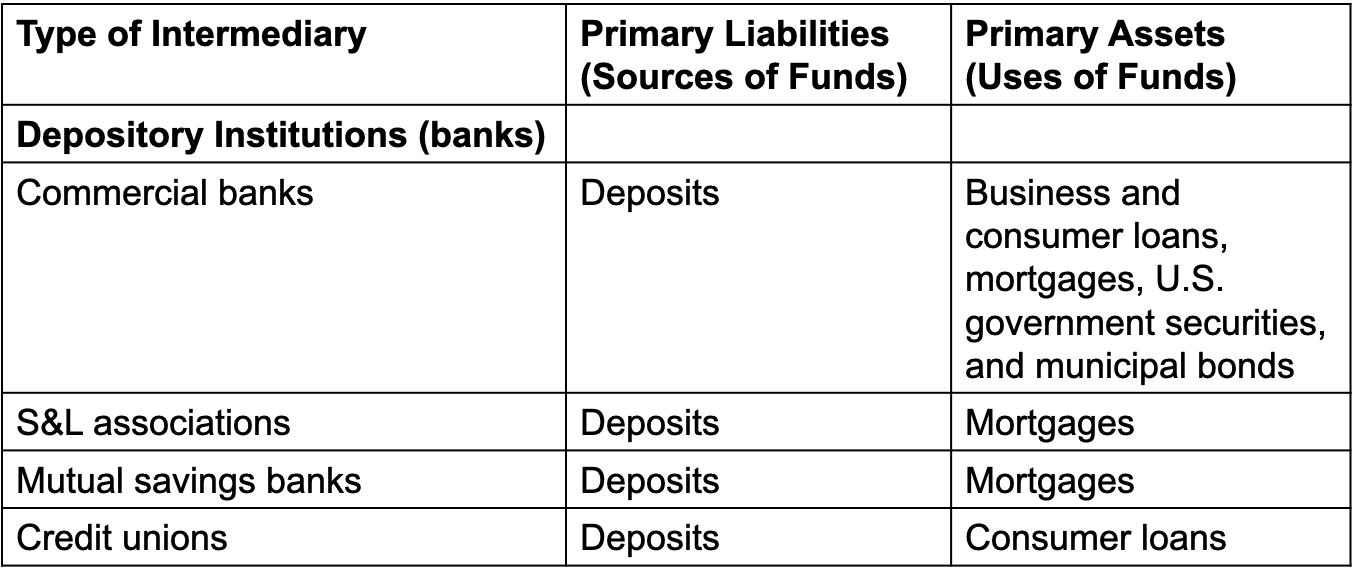
\includegraphics[height=6cm,width=11cm]{Picture4}
}

%------------------------------------------------

\frame
{
\frametitle{Primary Assets and Liabilities of Financial Intermediaries }
\centering 
\includegraphics[height=6cm,width=11cm]{Picture5}
}

%------------------------------------------------

\frame
{
\frametitle{Primary Assets and Liabilities of Financial Intermediaries}
\centering 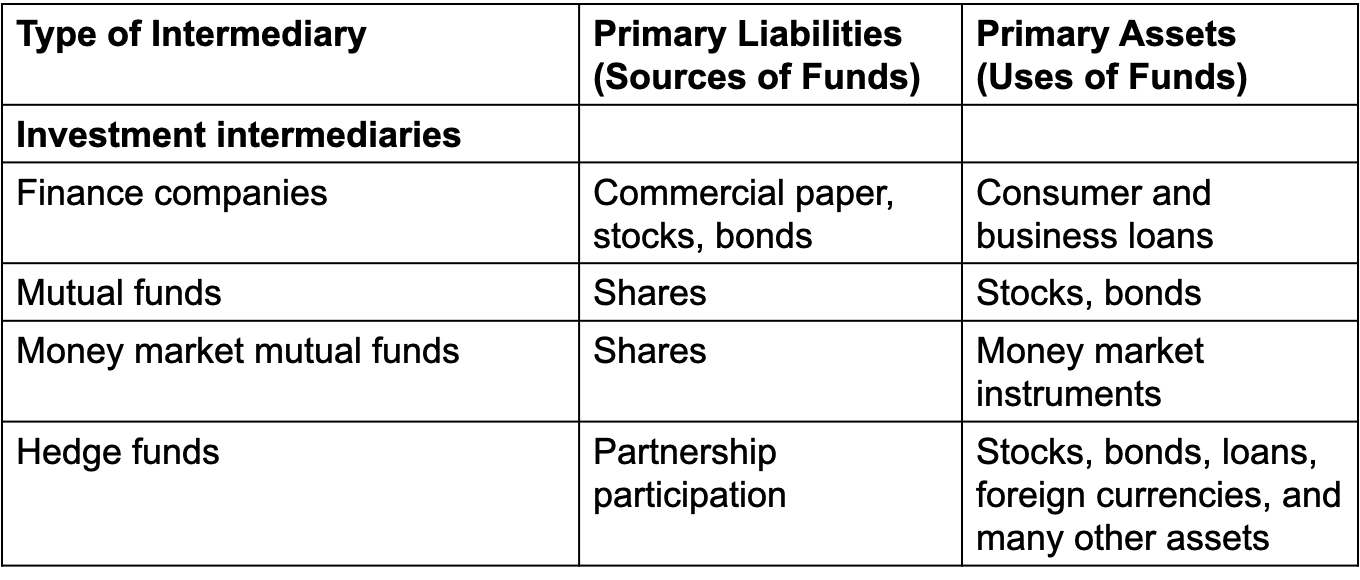
\includegraphics[height=6cm,width=11cm]{Picture6}
}



%------------------------------------------------
\begin{frame}
\frametitle{Regulation of Financial Markets}
Main Reasons for Regulation
\begin{enumerate}
\item Increase Information to Investors
\item Ensure the Soundness of Financial Intermediaries
\end{enumerate}

\end{frame}


%------------------------------------------------
\begin{frame}
\frametitle{Regulation Reason: Increase Investor Information }

\begin{itemize}
\item Asymmetric information in financial markets means that investors may be subject to adverse selection and moral hazard problems that may hinder the efficient operation of financial markets and may also keep investors away from financial markets.

\item The Securities and Exchange Commission (SEC) requires corporations issuing securities to disclose certain information about their sales, assets, and earnings to the public and restricts trading by the largest stockholders (known as insiders) in the corporation.

\item Such government regulation can reduce adverse selection and moral hazard problems in financial markets and increase their efficiency by increasing the amount of information available to investors. Indeed, the SEC has been particularly active recently in pursuing illegal insider trading.

\end{itemize}
\end{frame}

%------------------------------------------------
\begin{frame}
\frametitle{Regulation Reason: Ensure Soundness of Financial Intermediaries}

\begin{itemize}
\item To protect the public and the economy from financial panics, the government has implemented six types of regulations:

\begin{itemize}
\item Restrictions on Entry
\item Disclosure
\item Restrictions on Assets and Activities
\item Deposit Insurance
\item Limits on Competition
\item Restrictions on Interest Rates
\end{itemize}

\end{itemize}
\end{frame}

%------------------------------------------------
%\section{Conclusion}
%------------------------------------------------



\end{document} 